\documentclass[12pt, a4paper]{article}

% ── Encoding & language ──────────────────────────────────────
\usepackage[utf8]{inputenc}
\usepackage[T1]{fontenc}
\usepackage[italian]{babel}
\usepackage{lmodern}
\usepackage{microtype}
\usepackage{amsmath}

% ── Layout ───────────────────────────────────────────────────
\usepackage[margin=2.5cm, top=3cm, bottom=3cm]{geometry}
\setlength{\parskip}{5pt}
\setlength{\parindent}{0pt}

% ── Colors ───────────────────────────────────────────────────
\usepackage[dvipsnames]{xcolor}
\definecolor{primary}{RGB}{25, 90, 150}
\definecolor{light}{RGB}{235, 245, 255}
\definecolor{notebg}{RGB}{255, 252, 235}
\definecolor{noteborder}{RGB}{195, 155, 40}
\definecolor{quotebg}{RGB}{240, 245, 252}

% ── Section formatting ───────────────────────────────────────
\usepackage{titlesec}
\titleformat{\section}
  {\Large\bfseries\color{primary}}{}{0em}{}
  [\color{primary!50}\titlerule\vspace{2pt}]
\titleformat{\subsection}
  {\large\bfseries\color{primary!85}}{}{0em}{}
\titleformat{\subsubsection}
  {\normalsize\bfseries\color{primary!70}}{}{0em}{}
\titlespacing{\section}{0pt}{18pt}{6pt}
\titlespacing{\subsection}{0pt}{12pt}{4pt}
\titlespacing{\subsubsection}{0pt}{8pt}{2pt}

% ── Tables ───────────────────────────────────────────────────
\usepackage{booktabs}
\usepackage{tabularx}
\usepackage{array}
\usepackage{colortbl}
\renewcommand{\arraystretch}{1.25}

% ── Lists ────────────────────────────────────────────────────
\usepackage{enumitem}
\setlist[itemize]{topsep=3pt, itemsep=1pt, leftmargin=1.5em}
\setlist[enumerate]{topsep=3pt, itemsep=1pt, leftmargin=1.8em}

% ── Boxes ────────────────────────────────────────────────────
\usepackage{tcolorbox}
\tcbuselibrary{breakable, skins}

\newtcolorbox{notebox}[1][Nota]{
  colback=notebg,
  colframe=noteborder,
  arc=4pt,
  boxrule=1pt,
  title={\small\textbf{#1}},
  fonttitle=\bfseries\color{noteborder!80!black},
  breakable,
  left=8pt, right=8pt, top=4pt, bottom=4pt
}

\newtcolorbox{quotebox}{
  colback=quotebg,
  colframe=primary!30,
  arc=3pt,
  boxrule=0.6pt,
  left=10pt, right=10pt, top=4pt, bottom=4pt,
  breakable
}

\newtcolorbox{keybox}{
  colback=primary!8,
  colframe=primary!60,
  arc=4pt,
  boxrule=0.8pt,
  left=8pt, right=8pt, top=4pt, bottom=4pt,
  breakable
}

% ── Header / footer ──────────────────────────────────────────
\usepackage{fancyhdr}
\pagestyle{fancy}
\fancyhf{}
\fancyhead[L]{\small\textcolor{primary}{Istruttori FIN 2025 --- Riassunto per l'orale}}
\fancyhead[R]{\small\textcolor{primary}{\thepage}}
\renewcommand{\headrulewidth}{0.4pt}
\renewcommand{\headrule}{\color{primary!40}\hrule height 0.4pt}

% ── TOC ──────────────────────────────────────────────────────
\usepackage{tocloft}
\renewcommand{\cftsecfont}{\bfseries\color{primary}}
\renewcommand{\cftsubsecfont}{\small\color{primary!80}}
\renewcommand{\cftsecpagefont}{\bfseries\color{primary}}
\renewcommand{\cftsubsecpagefont}{\small\color{primary!80}}
\setlength{\cftbeforesecskip}{4pt}

% ── Hyperlinks ───────────────────────────────────────────────
\usepackage{hyperref}
\hypersetup{
  colorlinks=true,
  linkcolor=primary,
  urlcolor=primary,
  pdftitle={Riassunto per l'orale --- Istruttori FIN 2025},
  pdfauthor={FIN 2025},
}

% ─────────────────────────────────────────────────────────────
\begin{document}

\begin{center}
{\LARGE\bfseries\color{primary} Riassunto per l'Orale}\\[0.4em]
{\large\color{primary!80} Istruttori FIN 2025}
\end{center}

\vspace{0.8em}

\begin{quotebox}
Qui ho riportato la maggior parte dei concetti che \textit{potrebbe} chiedere all'esame orale, cose che Elia ha sottolineato durante le lezioni e il ripasso finale.
Buon studio.
\end{quotebox}

\vspace{1em}
\tableofcontents
\newpage

% ─────────────────────────────────────────────────────────────
\section{Cultura dell'acqua}

Scuola nuoto $\neq$ \textbf{Scuola di abilità acquatiche} $\rightarrow$ educare all'acqua attraverso l'acqua.

\textbf{Perché andare in piscina?} Non per imparare a nuotare, ma per acquisire determinate abilità per imparare a stare \textbf{\textit{bene}} in acqua.

\medskip
Sviluppo della personalità nelle sue diverse aree:

\medskip\noindent\textbf{Morfologico-funzionale}
\begin{itemize}
  \item Sviluppa strutture anatomiche, fisiologiche, biochimiche
  \item Previene difetti posturali e senso-motori
  \item Migliora percezione e consapevolezza ambientale
\end{itemize}

\noindent\textbf{Intellettivo-cognitiva}
\begin{itemize}
  \item Stimola SNC (cervello, cervelletto, tronco spinale)
  \item Migliora senso-percezione e immagine corporea
  \item Migliora prestazioni scolastiche e funzionamento quotidiano
\end{itemize}

\noindent\textbf{Affettivo-emotiva}
\begin{itemize}
  \item Occasione di socializzazione (vita sempre più strutturata, pochi coetanei)
  \item Previene squilibri affettivi e complessi
  \item Sviluppa autostima, percezione di sé, desiderio di autonomia
\end{itemize}

\noindent\textbf{Sociale}
\begin{itemize}
  \item Sviluppa senso di appartenenza
  \item Insegna rispetto regole e fiducia nella loro applicazione
  \item Sviluppa spirito di collaborazione ed emulazione
  \item Favorisce apprendimento cooperativo
\end{itemize}

\subsection{I Quattro Saperi dell'Istruttore}

\begin{tabularx}{\textwidth}{lX}
\toprule
\rowcolor{light} \textbf{Sapere} & \textbf{Descrizione} \\
\midrule
Sapere & Conoscenze teoriche legate al proprio ruolo: poche ma da avere ben chiare \\
Saper fare & Capacità pratica di riprodurre le tecniche richieste agli allievi e di intervenire in caso di necessità \\
Saper far fare & Comunicazione adeguata all'età e al grado di comprensione degli allievi per metterli in condizione di ottenere i risultati prefissati \\
Saper essere & Consapevolezza del proprio ruolo; essere ottimi osservatori e ascoltatori degli allievi per comprenderne le esigenze e trovare le soluzioni più adeguate per ciascuno \\
\bottomrule
\end{tabularx}

\subsection{Regole per la comunicazione}

\begin{enumerate}
  \item \textbf{Non si può non comunicare:} comunicazione e atteggiamenti assunti sono messaggi chiari agli allievi.
  \item \textbf{Il messaggio è sempre quello che arriva, non quello che parte}: se gli allievi non eseguono correttamente un esercizio, il problema non è che hanno capito male, ma che il linguaggio, il tono o la postura dell'istruttore non erano adeguati alle loro capacità di comprensione in quel momento.
\end{enumerate}

\subsection{I due concetti chiave}

\begin{keybox}
\textbf{Multilateralità}\\[2pt]
La \textbf{multilateralità} è la necessità di diversificare al massimo le esperienze motorie. Si sviluppa in due direzioni:
\begin{itemize}
  \item \textbf{Orizzontale}: fornire agli allievi il maggior numero possibile di esperienze motorie per stimolare il sistema nervoso centrale a trovare sempre strade e soluzioni differenti a qualsiasi tipo di problema motorio.
  \item \textbf{Verticale}: varie condizioni di \textbf{velocità, ritmo e ampiezza} di movimento.
\end{itemize}
\end{keybox}

\begin{keybox}
\textbf{Sensopercezione}\\[2pt]
La \textbf{senso percezione} è il processo attraverso il quale il corpo percepisce e interpreta le informazioni che l'ambiente fornisce attraverso i cinque sensi, le integra e le traduce in movimento. Equivale alla consapevolezza della posizione del proprio corpo nell'acqua e del modo in cui l'acqua reagisce al movimento.
\end{keybox}

\subsection{Fase Sensibile}

Il periodo tra i \textbf{6 e 14 anni} circa $\rightarrow$ \textbf{fase sensibile dello sviluppo coordinativo}.
Il sistema nervoso e l'apparato muscolo-scheletrico sono in una fase di sviluppo che permette l'acquisizione ottimale di nuove competenze motorie.

\begin{itemize}
  \item Sviluppo delle capacità coordinative attorno ai \textbf{6--12 anni}.
  \item \textbf{Pre-adolescenza e pubertà in poi}: inizio del lavoro significativo sulle capacità condizionali.
\end{itemize}

\begin{figure}[h]
    \centering
    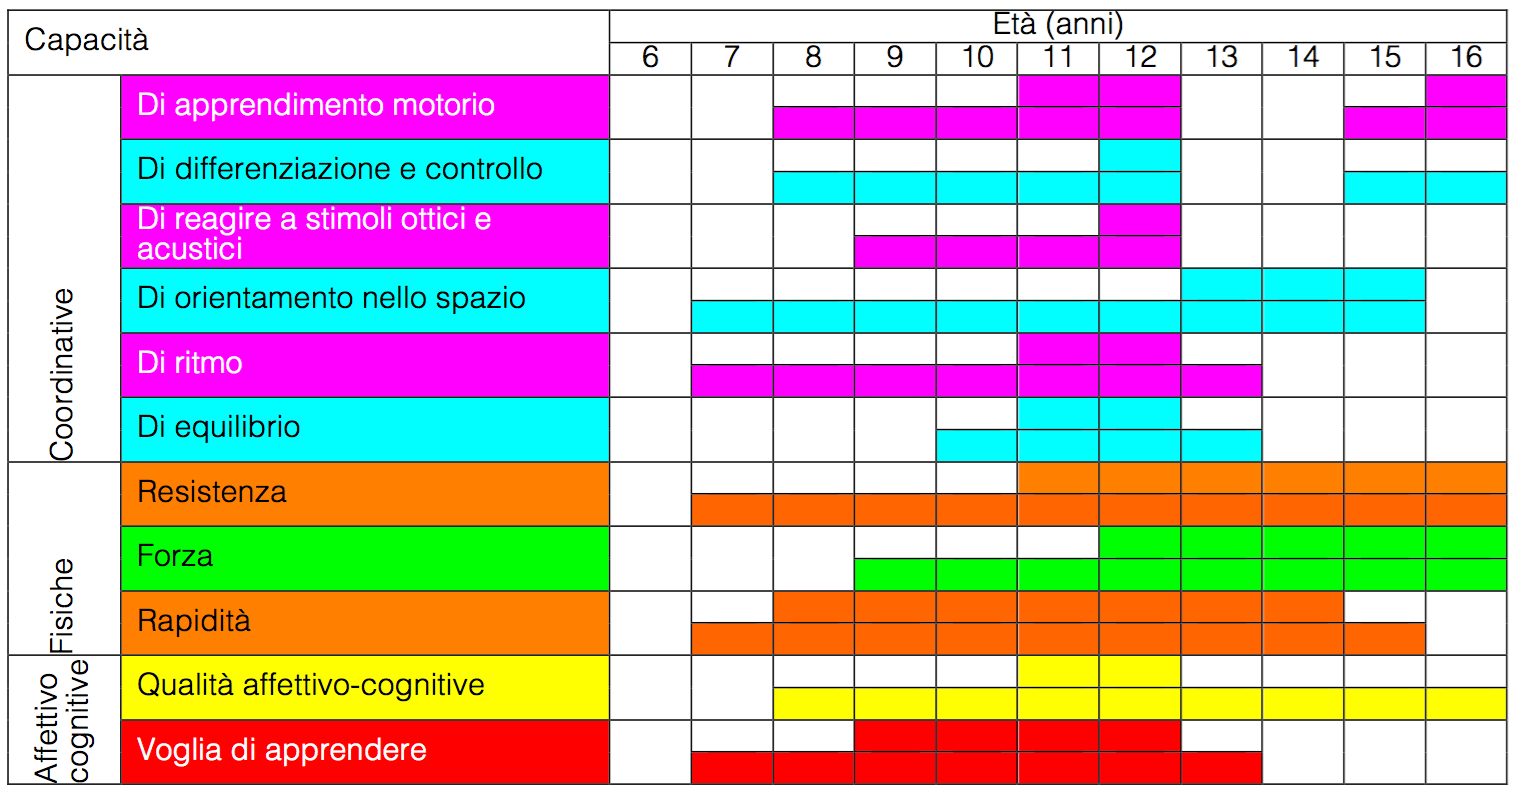
\includegraphics[width=1.0\textwidth]{Pics/Pasted image 20260309105712.png}
    \caption{Fase sensibile dello sviluppo coordinativo}
    \label{fig:fase_sensibile}
\end{figure}

\subsection{Proprietà dell'acqua}

\subsubsection{Resistenza dell'acqua}
\begin{itemize}
  \item \textbf{800 volte superiore} a quella dell'aria
  \item Muoversi con efficacia $\rightarrow$ \textbf{ridurre le resistenze} e aumentare le propulsioni
  \item Resistenza è \textbf{progressiva}: aumenta con il quadrato della velocità $\rightarrow$ posizione del corpo fondamentale
\end{itemize}

\subsubsection{Spinta idrostatica}

Unico elemento utile al movimento in acqua.
\textbf{Principio di Archimede} $\rightarrow$ un corpo immerso in un liquido riceve una spinta verso l'alto proporzionale alla quantità di liquido spostato.

Conseguenze:
\begin{itemize}
  \item Spinta idrostatica massima $\rightarrow$ \textbf{posizione orizzontale} del corpo.
  \item \textbf{Rilassare la muscolatura} per distendere il peso del corpo sulla porzione di acqua più ampia possibile.
\end{itemize}

% ─────────────────────────────────────────────────────────────
\section{Teoria del movimento}

Le capacità motorie sono i presupposti delle azioni motorie --- le potenzialità di un individuo. Si dividono in \textbf{coordinative}, \textbf{condizionali} e \textbf{mobilità articolare}.

\subsection{Capacità coordinative}

Sono legate al \textbf{sistema nervoso} --- lato cognitivo del movimento. Divise in \textbf{generali} e \textbf{speciali}.

\subsubsection{Capacità coordinative generali}

Sono tre:
\begin{enumerate}
  \item \textbf{Capacità di apprendimento}: prima imparo il movimento.
  \begin{enumerate}
    \item \textbf{Coordinazione grezza}: prima esecuzione imperfetta, migliora ripetendo correttamente il movimento.
    \item \textbf{Coordinazione fine}: il movimento diventa sempre più dettagliato, preciso, efficace.
    \item \textbf{Disponibilità variabile}: ultima fase, il movimento viene ulteriormente affinato e può essere eseguito in qualsiasi condizione.
  \end{enumerate}
  \item \textbf{Capacità di controllo}: precisione esecutiva di una determinata abilità.
  \item \textbf{Capacità di adattamento e trasformazione}: adattare il movimento alle diverse situazioni.
\end{enumerate}

\subsubsection{Capacità coordinative speciali}

\begin{tabularx}{\textwidth}{lX}
\toprule
\rowcolor{light} \textbf{Tipo} & \textbf{Descrizione} \\
\midrule
Ritmo & Scelta temporale degli impulsi per realizzare in modo adeguato un'azione finalizzata \\
Reazione & Elaborazione rapida dello stimolo percettivo $\Rightarrow$ velocità di trasmissione degli organi recettori \\
Equilibrio & Mantenere postura utile all'azione (vestibolare) \\
Orientamento & Mantenere il giusto rapporto con il campo d'azione e i riferimenti spaziali \\
Combinazione motoria & Coordinazione di più movimenti \\
Differenziazione cinestesica & Dosare forza per massima efficacia \\
Anticipazione motoria & Previsione, pre-costituzione dell'azione successiva \\
Fantasia motoria & Usare abilità apprese per risolvere un problema motorio \\
\bottomrule
\end{tabularx}

\subsection{Capacità condizionali}

\begin{enumerate}
  \item \textbf{Forza}: capacità di vincere, opporsi a una resistenza con un impegno tensivo del muscolo.
  \begin{enumerate}
    \item \textbf{Forza massimale}: massima tensione volontaria (si allena dai 16--17 anni).
    \item \textbf{Forza resistente}: dipendente da sistema muscolare e apparati cardio-circolatorio. Forza che si protrae nel tempo (da 11--12 anni).
    \item \textbf{Forza veloce}: intensità elevata nel minor tempo possibile (da 8 anni, per maggior presenza di fibre bianche).
  \end{enumerate}
  \item \textbf{Resistenza}: capacità di sopportare o prolungare per il maggior tempo possibile uno sforzo.
  \begin{itemize}
    \item Motivazione --- Efficacia del gesto --- Ritmo
  \end{itemize}
  \item \textbf{Velocità}: eseguire un gesto nel minor tempo possibile. Legata a: fattori psicologici, fattori nervosi, quantità di fibre bianche, corretta tecnica del gesto motorio.
\end{enumerate}

Ordine corretto di stimolazione: \textbf{velocità $\rightarrow$ forza $\rightarrow$ resistenza}.

Il bambino ha fibre muscolari \textbf{bianche} (veloci) in prevalenza, che con l'età si trasformano in \textbf{rosse} (resistenti). La fase sensibile della velocità è la più precoce: 6--8 anni.

La forza in acqua è già stimolata dalla densità (\textbf{800$\times$ superiore all'aria}). Importante anche negli anziani per prevenire la \textbf{sarcopenia}.

\subsection{Mobilità articolare}

Capacità intermedia con forte componente ereditaria. Per le fasce di età della scuola nuoto non è necessario un lavoro specifico: gli esercizi del nuoto richiedono già una grande ampiezza di movimento.

\subsection{Fattori della prestazione}

La prestazione è l'esito misurabile di un'azione sportiva completa. Dipende da 4 fattori:
\begin{itemize}
  \item \textbf{Costituzione}: massa corporea, segmenti corporei, mobilità articolare.
  \item \textbf{Condizione}: sviluppo delle capacità condizionali (grandi apparati: muscolo-scheletrico, cardio-circolatorio).
  \item \textbf{Coordinazione}: controllo e regolazione del movimento.
  \item \textbf{Controllo}: processi emotivi, cognitivi e motivazionali.
\end{itemize}

\subsection{Analizzatori}

La sensopercezione è legata agli \textbf{analizzatori}: strutture funzionali che selezionano, codificano e trasmettono stimoli al sistema nervoso.

\begin{itemize}
  \item \textbf{Esterocettori}: acustico, ottico, tattile.
  \item \textbf{Propriocettori}:
  \begin{itemize}
    \item \textbf{Cinestesico}: fusi neuromuscolari e organi tendinei $\rightarrow$ informazioni relative al movimento.
    \item \textbf{Vestibolare}: nell'orecchio interno, segnali legati ai movimenti nello spazio.
  \end{itemize}
\end{itemize}

Regola base dell'insegnamento: \textbf{globale prima, analitico dopo. Sempre.}

\subsection{Sviluppo del bambino e schema corporeo}

Nella fascia prescolare (3--4 anni) si costruisce lo \textbf{schema corporeo} --- la consapevolezza di avere un corpo. A 5--6 anni di solito è già consolidato.

Dopodiché vengono gli \textbf{schemi motori di base terrestri}: camminare, correre, saltare, arrampicarsi, lanciare, rotolare. In acqua questi schemi diventano più difficili ma vanno comunque stimolati.

Le \textbf{abilità} si costruiscono combinando più schemi motori. Saltare è uno schema motorio di base; fare un tuffo è un'abilità.

\subsubsection{Turgor e Proceritas}

\begin{itemize}
  \item \textbf{Turgor}: si allarga (accumula riserve prima di allungarsi).
  \item \textbf{Proceritas}: si allunga.
\end{itemize}

Schema tipico: piccolo e ciccio $\rightarrow$ si allunga $\rightarrow$ verso 8--9 anni si allarga $\rightarrow$ si allunga ancora $\rightarrow$ fase post-adolescenziale.

\subsection{Disabilità}

Disabilità motoria e cognitiva/emotiva si trascinano a vicenda. Una disabilità motoria dalla nascita limita le esperienze $\rightarrow$ ricadute cognitive, relazionali, emotive. Vale anche al contrario. Le difficoltà però si possono recuperare.

% ─────────────────────────────────────────────────────────────
\section{Elementi di Primo Soccorso}

\subsection{Regole generali}

\begin{itemize}
  \item Chiamare \textbf{112} sempre per primo (omissione di soccorso = reato penale, art.\ 593 c.p.)
  \item Non mettere a rischio la propria sicurezza
  \item Non spostare mai il traumatizzato (rischio paralisi) --- eccezione: pericolo di vita immediato
  \item Non somministrare nulla per bocca
  \item Indossare \textbf{guanti in lattice} in presenza di sangue (epatite B/C, HIV non richiedono certificazione per accedere agli impianti)
\end{itemize}

\subsection{Disturbi della coscienza}

\begin{itemize}
  \item \textbf{Lipotemia}: malessere passeggero, si risolve da solo.
  \item \textbf{Sincope}: perdita di coscienza con caduta $\rightarrow$ sollevare gambe $\sim$30 cm, slacciare indumenti stretti, non somministrare nulla. Se arresto cardiocircolatorio $\rightarrow$ BLS + DAE.
\end{itemize}

\subsection{Epilessia}

Interessa il \textbf{2\% della popolazione} --- anche atleti con idoneità agonistica possono essere epilettici.

\begin{itemize}
  \item Attacco di grande male dura \textbf{1--2 minuti}, poi fase di sonno profondo (il soggetto non ricorda nulla).
  \item \textbf{Fare}: posizione laterale di sicurezza, materiale morbido sotto la testa, slacciare indumenti, annotare il tempo, non lasciarlo solo, verificare polso e respiro.
  \item \textbf{Non fare}: non bloccare le scosse, non aprire la bocca con la forza, non usare il cuneo apribocca (responsabilità civile).
\end{itemize}

\subsection{Emorragie}

\begin{tabularx}{\textwidth}{lX}
\toprule
\rowcolor{light} \textbf{Tipo} & \textbf{Caratteristiche} \\
\midrule
Arteriosa & Rosso vivo, schizzi pulsanti --- molto grave \\
Venosa & Rosso scuro, flusso continuo --- più frequente \\
Capillare & Stilla, si arresta da sola --- lieve \\
Interna esteriorizzata & Da orifizi naturali --- \textbf{non tamponare} \\
\bottomrule
\end{tabularx}

\medskip
\textbf{Esterne}: compressione con garze + non rimuovere tampone + bendaggio compressivo + ghiaccio + ospedale.\\
\textbf{Interne gravi} (trauma addominale, frattura bacino): chiamare 112 subito.

\subsection{Lesioni muscolari --- RICE (prime 48h)}

\begin{tabular}{ll}
\toprule
\rowcolor{light} \textbf{Lettera} & \textbf{Significato} \\
\midrule
\textbf{R} & \textit{Rest} --- riposo immediato \\
\textbf{I} & \textit{Ice} --- ghiaccio \\
\textbf{C} & \textit{Compression} --- bendaggio compressivo \\
\textbf{E} & \textit{Elevation} --- arto sollevato \\
\bottomrule
\end{tabular}

\medskip
Ghiaccio: 20 min ogni 2--4h per 3--4 giorni. Massaggi solo dopo \textbf{una settimana}. Farmaci = competenza medica.

\subsection{Lussazione}

Perdita permanente del contatto articolare. \textbf{Non rimettere a posto} (competenza ortopedica; responsabilità civile). Immobilizzare, ghiaccio, controllare circolo a valle, ospedale.

\subsection{Fratture}

Non spostare il soggetto. Non rimuovere oggetti conficcati (fanno da tappo). Fratture esposte: telino sterile + soluzione fisiologica.

\subsection{BLS --- Basic Life Support}

\textbf{Diagnosi}: soggetto non cosciente + assenza di respiro. Ricerca del polso \textbf{abolita dal 2005}.

Catena della sopravvivenza:
\begin{enumerate}
  \item Prevenzione
  \item Accesso precoce al 112
  \item RCP precoce (compressioni + ventilazioni)
  \item Defibrillazione precoce (DAE)
  \item Soccorso avanzato con farmaci (solo personale sanitario)
\end{enumerate}

\textbf{DAE}: la macchina decide se scaricare. Il soccorritore garantisce solo la sicurezza. Formula: \textbf{``via io, via tu, via tutti''} prima dell'analisi. Obbligatorio per legge in tutti gli impianti sportivi.

\subsection{Ostruzione vie aeree --- Manovra di Heimlich}

\begin{itemize}
  \item \textbf{Parziale} (tossisce ancora): incoraggiare a tossire, non intervenire.
  \item \textbf{Totale cosciente}: 5 pacche sulla schiena $\rightarrow$ se non basta: manovra di Heimlich (spinte dal basso verso l'alto sotto l'arcata costale).
  \item \textbf{Non cosciente}: BLS standard; dopo ogni 30 compressioni verificare se il corpo estraneo è visibile in bocca.
\end{itemize}

% ─────────────────────────────────────────────────────────────
\section{Il Corpo Umano}

\subsection{Cellula: strutture chiave}

\begin{itemize}
  \item \textbf{Membrana cellulare}: proteine + fosfolipidi; selettiva --- regola cosa entra e cosa esce.
  \item \textbf{Nucleo}: contiene il \textbf{DNA}.
  \item \textbf{Mitocondri}: producono \textbf{energia}.
  \item Cellule muscolari: ricche di mitocondri + proteine contrattili (actina, miosina).
\end{itemize}

\subsection{Quattro sistemi connessi con il movimento}

\begin{enumerate}
  \item \textbf{Sistema nervoso} (centrale + periferico): ordini motori + informazioni dalla periferia.
  \item \textbf{Apparato respiratorio}: porta O\textsubscript{2} dentro, butta CO\textsubscript{2} fuori.
  \item \textbf{Apparato cardiocircolatorio}: trasporta O\textsubscript{2} ai tessuti.
  \item \textbf{Apparato osteoarticolare + muscolare}: eseguono il movimento.
\end{enumerate}

\subsection{Riserve energetiche}

\begin{tabularx}{\textwidth}{lXl}
\toprule
\rowcolor{light} \textbf{Substrato} & \textbf{Deposito} & \textbf{Dove} \\
\midrule
Zuccheri & Glicogeno & Fegato e muscolo \\
Grassi & Tessuto adiposo & Prevalentemente sottocutaneo \\
Proteine & Nessun deposito & Solo circolanti/strutturali \\
\bottomrule
\end{tabularx}

\subsection{Tre meccanismi energetici}

\begin{tabularx}{\textwidth}{lXX}
\toprule
\rowcolor{light} \textbf{Meccanismo} & \textbf{Substrato} & \textbf{Note} \\
\midrule
\textbf{Anaerobico alattacido} & Fosfocreatina + ATP & Rapidissimo, brevissima durata, no acido lattico \\
\textbf{Anaerobico lattacido} & Zuccheri $\rightarrow$ acido lattico & Rapido, durata limitata \\
\textbf{Aerobico} & Grassi/zuccheri + O\textsubscript{2} & Predominante a lungo termine; O\textsubscript{2} va rifornito in continuo \\
\bottomrule
\end{tabularx}

\subsection{Sistema nervoso}

\textbf{SNC}: cervello + cervelletto (nella scatola cranica) + midollo spinale (nella colonna vertebrale).

\textbf{Sistema nervoso periferico}:
\begin{itemize}
  \item \textbf{Motoneuroni} (efferenti): SNC $\rightarrow$ muscoli (ordini di contrazione).
  \item \textbf{Nervi della sensibilità} (afferenti): periferia $\rightarrow$ cervello (dolore, temperatura, posizione).
\end{itemize}

\textbf{Cosciente vs automatico}:
\begin{itemize}
  \item Stimoli alla \textbf{corteccia cerebrale} $\rightarrow$ azioni volontarie.
  \item Stimoli al \textbf{cervelletto} $\rightarrow$ postura ed equilibrio \textbf{automatici}.
\end{itemize}

\textbf{Sistema nervoso autonomo} (simpatico/parasimpatico):

\begin{tabularx}{\textwidth}{lXX}
\toprule
\rowcolor{light} & \textbf{Simpatico} & \textbf{Parasimpatico} \\
\midrule
FC & Aumenta & Diminuisce \\
Bronchi & Dilata & Contringe \\
Attivato da & Stress, paura, caffeina, ormoni surrenali & Riposo \\
\bottomrule
\end{tabularx}

\textbf{Apprendimento motorio}: un gesto nuovo deve passare per la coscienza. Una volta memorizzato diventa \textbf{semi-automatico}. Il nuoto non è un gesto naturale: va imparato.

\subsection{Apparato respiratorio}

\begin{figure}[h]
    \centering
    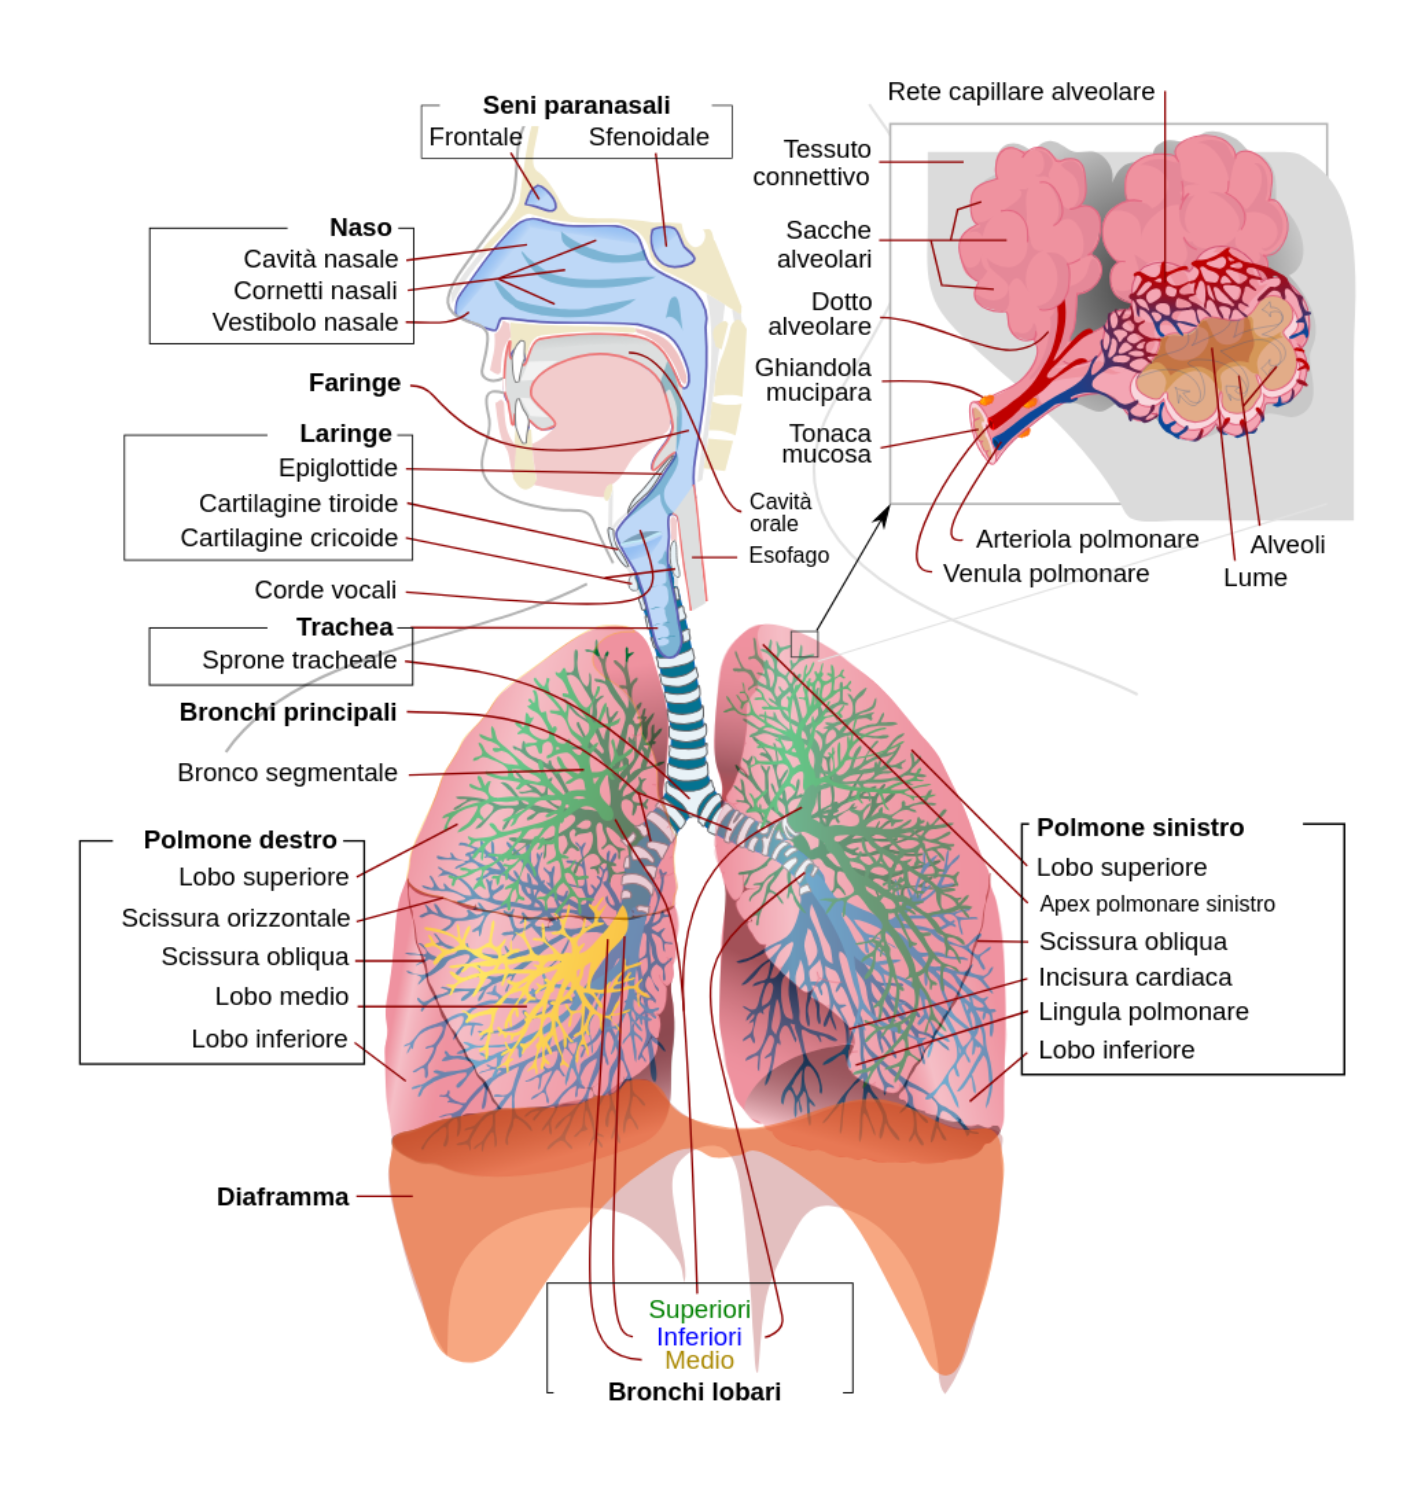
\includegraphics[width=0.8\textwidth]{Pics/Drawing 2026-04-14 15.48.28.excalidraw.png}
    \caption{Apparato respiratorio}
    \label{fig:respiratorio}
\end{figure}

Percorso dell'aria: \textbf{naso/bocca $\rightarrow$ faringe $\rightarrow$ laringe} (corde vocali) \textbf{$\rightarrow$ trachea} (anelli cartilaginei) \textbf{$\rightarrow$ bronchi $\rightarrow$ bronchioli $\rightarrow$ alveoli}.

Negli \textbf{alveoli}: O\textsubscript{2} passa dall'aria al sangue; CO\textsubscript{2} passa dal sangue all'aria.

\textbf{Meccanica}:
\begin{itemize}
  \item \textbf{Inspirazione}: diaframma (abbassa) + intercostali (alzano le coste) $\rightarrow$ pressione negativa $\rightarrow$ aria entra.
  \item \textbf{Espirazione a riposo}: passiva (rilascio + forza elastica).
  \item \textbf{Espirazione forzata}: muscoli attivi; sforzo massimale: anche muscoli accessori del collo.
\end{itemize}

\textbf{Parametri}:

\begin{tabular}{llll}
\toprule
\rowcolor{light} & \textbf{Atti/min} & \textbf{Volume/atto} & \textbf{Totale} \\
\midrule
Riposo & $\sim$12 & $\sim$0,5 L & $\sim$6 L/min \\
Sforzo max & 40--50 & fino a 5 L & 150+ L/min ($\sim$25$\times$ il riposo) \\
\bottomrule
\end{tabular}

\textbf{Debito di ossigeno}: lavoro anaerobico produce prodotti che richiedono O\textsubscript{2} per essere smaltiti $\rightarrow$ l'affanno dopo lo sforzo dura più a lungo. La durata dell'affanno è \textbf{indicatore di quanto è stato intenso il lavoro anaerobico}.

\subsection{Apparato cardiocircolatorio}

Sistema \textbf{chiuso a doppio circuito}. Cuore = 4 cavità: \textbf{atri} (dx e sx, ricevono il sangue) e \textbf{ventricoli} (dx e sx, pompano il sangue).

\begin{tabularx}{\textwidth}{lXX}
\toprule
\rowcolor{light} \textbf{Circuito} & \textbf{Percorso} & \textbf{Funzione} \\
\midrule
\textbf{Polmonare} (piccolo) & Ventricolo dx $\rightarrow$ polmoni $\rightarrow$ atrio sx & Ossigenazione \\
\textbf{Sistemico} (grande) & Ventricolo sx $\rightarrow$ aorta $\rightarrow$ tessuti $\rightarrow$ atrio dx & Distribuzione O\textsubscript{2} \\
\bottomrule
\end{tabularx}

\subsubsection{Quattro valvole cardiache}

\begin{figure}[h]
    \centering
    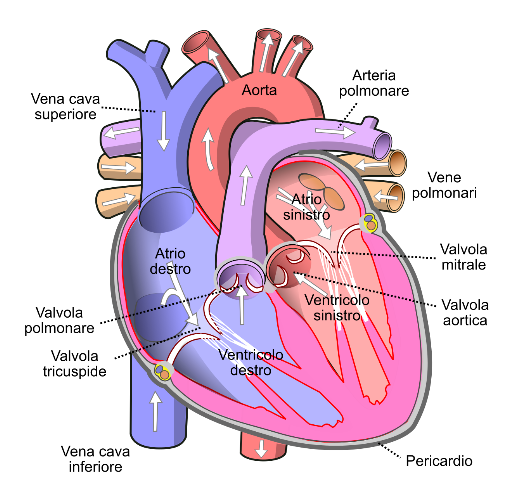
\includegraphics[width=0.8\textwidth]{Pics/Drawing 2026-04-14 15.43.14.excalidraw.png}
    \caption{Quattro valvole cardiache}
    \label{fig:valvole}
\end{figure}

\begin{tabularx}{\textwidth}{lX}
\toprule
\rowcolor{light} \textbf{Valvola} & \textbf{Posizione} \\
\midrule
\textbf{Mitrale} (bicuspide) & Atrio sx $\rightarrow$ ventricolo sx \\
\textbf{Tricuspide} & Atrio dx $\rightarrow$ ventricolo dx \\
\textbf{Semilunare aortica} & Ventricolo sx $\rightarrow$ aorta \\
\textbf{Semilunare polmonare} & Ventricolo dx $\rightarrow$ arteria polmonare \\
\bottomrule
\end{tabularx}

Una valvola lesionata = sangue refluisce = \textbf{cuore lavora doppio}.

\subsubsection{Parametri cardiaci}

\begin{tabular}{lll}
\toprule
\rowcolor{light} & \textbf{Riposo} & \textbf{Sforzo massimale} \\
\midrule
FC & $\sim$60 bpm & 150--200 bpm \\
Volume sistolico & $\sim$60 cc & $\sim$100 cc \\
Portata & $\sim$3,6 L/min & 15--20 L/min ($\sim$4--5$\times$) \\
\bottomrule
\end{tabular}

\begin{quotebox}
Il sistema respiratorio aumenta 25$\times$, quello cardiovascolare solo 4--5$\times$: è il cardiovascolare il \textbf{fattore limitante} nel trasporto di O\textsubscript{2}.
\end{quotebox}

\textbf{FC massimale = 220 $-$ età.} \quad
Pulsazioni: arteria \textbf{radiale} (polso) o \textbf{carotide} (collo).\\
\textbf{Pressione normale}: 120/70 mmHg.\quad
\textbf{Soglia aerobica/anaerobica}: $\sim$70--80\% della FC massimale.

\subsection{Apparato locomotore}

Articolazioni: \textbf{fissa} (cranio), \textbf{semimobile} (vertebre), \textbf{uniplanare} (ginocchio), \textbf{multidirezionale} (spalla --- massima mobilità, massimi infortuni nei nuotatori).

\subsection{Struttura e contrazione muscolare}

Proteine contrattili: \textbf{actina} (filamento sottile) + \textbf{miosina} (filamento spesso con ponti crociati).

Catena dello stimolo: cervello $\rightarrow$ segnale elettrico (motoneurone) $\rightarrow$ sinapsi chimica $\rightarrow$ ioni calcio $\rightarrow$ ATP $\rightarrow$ ADP + energia $\rightarrow$ actina scivola su miosina.

Struttura gerarchica: actina+miosina $\rightarrow$ miofibrille $\rightarrow$ cellula muscolare $\rightarrow$ fascio di fibre $\rightarrow$ muscolo scheletrico.

Muscoli principali della bracciata: \textbf{pettorale} e \textbf{gran dorsale}.

\subsection{Leve nel corpo umano}

\begin{tabularx}{\textwidth}{llX}
\toprule
\rowcolor{light} \textbf{Specie} & \textbf{Caratteristica} & \textbf{Esempio} \\
\midrule
Seconda & \textbf{Vantaggiosa} (poca forza $\rightarrow$ grande resistenza) & Alzarsi sulle punte dei piedi \\
Terza & \textbf{Svantaggiosa} in forza, vantaggiosa in escursione & Bracciata del nuoto (escursione 1,5--1,8 m) \\
\bottomrule
\end{tabularx}

La \textbf{maggior parte delle leve del corpo} sono di \textbf{terza specie}.

\subsection{Tipi di contrazione}

\begin{tabularx}{\textwidth}{llX}
\toprule
\rowcolor{light} \textbf{Tipo} & \textbf{Cosa fa il muscolo} & \textbf{Esempio} \\
\midrule
\textbf{Concentrica} & Si contrae e si \textbf{accorcia} & Sollevare un peso (bicipite) \\
\textbf{Eccentrica} & Si contrae ma si \textbf{allunga} & Atterraggio dopo un salto \\
\textbf{Isometrica} & Si contrae, \textbf{nessun movimento} & Spingere su una parete fissa \\
\bottomrule
\end{tabularx}

La \textbf{eccentrica} è la più stressante --- i carichi possono superare la forza massimale concentrica.

Il \textbf{nuoto si avvicina all'isocinetico} perché la resistenza dell'acqua smorza accelerazioni e decelerazioni.

% ─────────────────────────────────────────────────────────────
\section{Psicopedagogia}

\subsection{Comunicazione}

\begin{figure}[h]
  \centering
  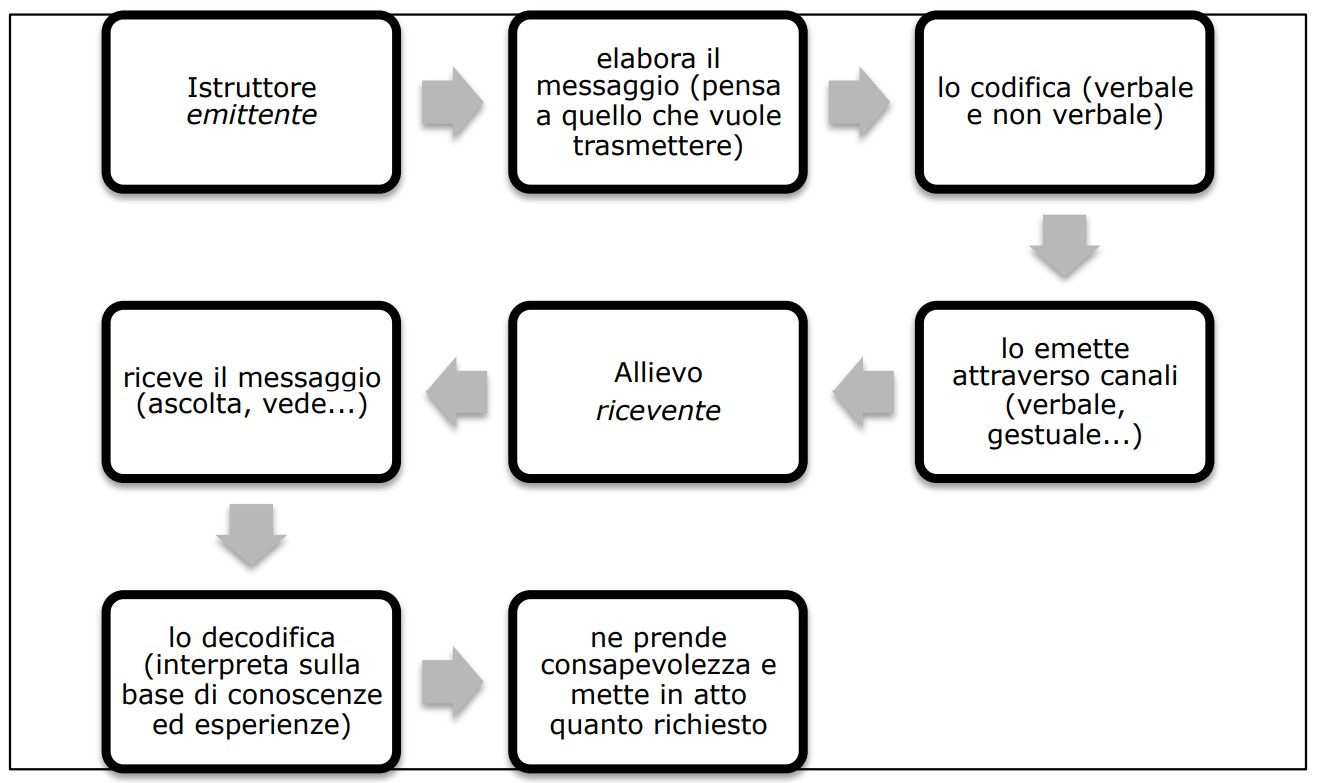
\includegraphics[width=0.8\textwidth]{Pics/Pasted image 20260309105803.png}
  \caption{Comunicazione}
  \label{fig:comunicazione}
\end{figure}

La comunicazione è \textbf{bidirezionale}: istruttore e allievo sono al tempo stesso emittenti e riceventi. Principio chiave: \textbf{conta ciò che arriva, non ciò che parte}. Il codice \textbf{non verbale} (come si dice) pesa più di quello verbale (cosa si dice): postura, tono di voce, sguardo, gestualità.

In piscina ci sono molte barriere (rumore, affollamento): serve una \textbf{gestualità condivisa} e \textbf{regole di ingaggio} chiare.

\subsection{Intelligenza emotiva}

Introdotta da \textbf{Salovey e Mayer (1990)}, resa popolare da \textbf{Goleman (1995)}. Cinque ambiti:
\begin{enumerate}
  \item Riconoscere le proprie emozioni
  \item Padroneggiare le proprie emozioni
  \item Motivare se stessi
  \item Riconoscere le emozioni altrui
  \item Utilizzare le competenze sociali
\end{enumerate}

Negli istruttori è fondamentale il punto 4 --- capire umore, temperamento e motivazione di ciascun allievo.

\subsection{Apprendimento}

\begin{itemize}
  \item \textbf{Piaget}: ruolo dell'imitazione.
  \item \textbf{Bandura}: \textit{modeling} --- apprendimento per osservazione di un modello.
  \item \textbf{Vygotsky}: \textbf{zona di sviluppo prossimale} --- ciò che il bambino non riesce a fare da solo ma riesce con l'aiuto degli altri. È lì che l'istruttore deve agire.
\end{itemize}

L'esperienza è la condizione imprescindibile per l'apprendimento.

\subsection{Autostima}

\begin{figure}[h]
  \centering
  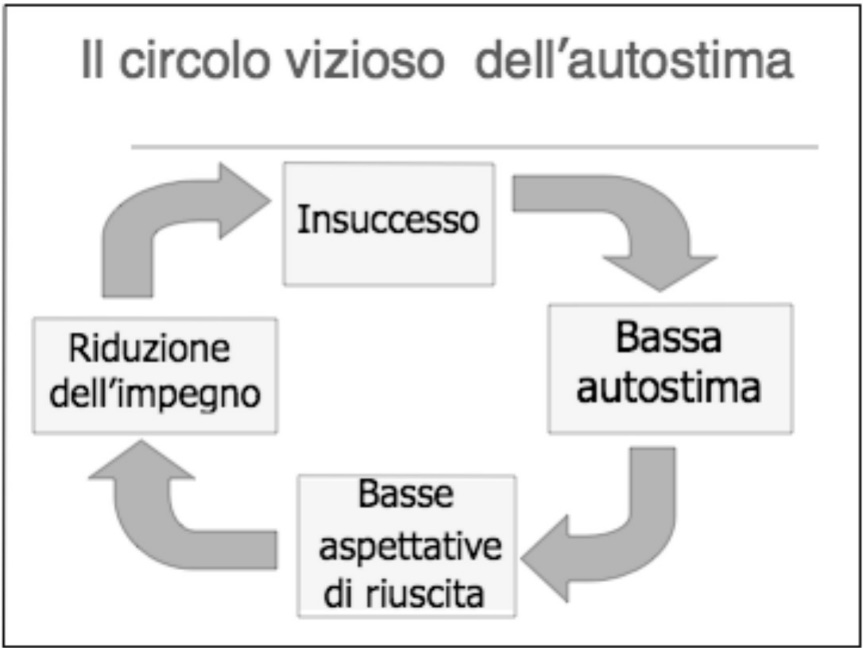
\includegraphics[width=0.65\textwidth]{Pics/Pasted image 20260309105909.png}
  \caption{Autostima}
  \label{fig:autostima}
\end{figure}

Interazione tra \textbf{sé reale} (ciò che si è) e \textbf{sé ideale} (ciò che si vorrebbe essere). Maggiore la discrepanza $\rightarrow$ minore l'autostima.

L'istruttore deve:
\begin{itemize}
  \item Sottolineare i successi $\rightarrow$ rinforza il \textbf{senso di autoefficacia}.
  \item Usare la \textbf{critica costruttiva}: criticare sempre il \textbf{comportamento}, mai la persona.
  \item Proporre \textbf{obiettivi raggiungibili} con il giusto grado di fatica.
  \item Incoraggiare il \textbf{dialogo interno positivo}: ``ce la posso fare''.
\end{itemize}

\subsection{Gestione del gruppo}

Il gruppo è un sistema complesso --- non è la somma dei suoi componenti. La conduzione deve essere \textbf{intenzionale, sistematica e flessibile}.

Le regole devono essere \textbf{poche, chiare e stabili}: clima troppo protettivo $\rightarrow$ dipendenza; clima lassista $\rightarrow$ insicurezza.

\subsection{Fasce d'età}

\subsubsection{Adolescente}

La \textit{proceritas secunda} scatena una \textbf{tempesta ormonale} (\textit{vagotonia}): lo schema corporeo diventa \textbf{disarmonico e sgraziato}. L'allievo percepisce una perdita di efficacia nella nuotata --- causa frequente di abbandono. L'istruttore deve \textbf{informarlo e renderlo consapevole} che è temporaneo.

\begin{itemize}
  \item \textbf{Locus of control interno}: l'allievo capisce di poter incidere sui propri risultati.
  \item \textbf{Resilienza}: capacità di affrontare le avversità --- lo sport è il contesto ideale per svilupparla.
\end{itemize}

\subsubsection{Adulto e anziano}

I cambiamenti fisiologici sono reali ma \textbf{non sono patologia}. L'esercizio fisico stimola la produzione di \textbf{beta-endorfine} (tolleranza al dolore, riduzione ansia, benessere). Il pensionamento è un momento di rischio sociale: il gruppo sportivo è un antidoto.

\textbf{Socializzazione trasversale}: favorire l'integrazione tra fasce d'età diverse.

% ─────────────────────────────────────────────────────────────
\section{Le 4 nuotate fondamentali}

Il modello prestativo serve per leggere il gesto dell'allievo e capire dove si discosta dall'ideale.

\textbf{Continuità}, \textbf{ampiezza} e \textbf{traiettoria} (mani vicino al corpo) sono i tre parametri trasversali a tutti gli stili. La spinta finale va sempre in forte accelerazione crescente. Ascella aperta nella presa, sempre.

\subsection{Stile libero}

Asimmetrico, alto rendimento meccanico, con rollio (parte dai fianchi, la testa rimane in asse). Tollera gli errori coordinativi nelle fasi iniziali --- da proporre per primo.

Passata subacquea: appoggio/presa $\rightarrow$ trazione $\rightarrow$ spinta in forte accelerazione $\rightarrow$ recupero (inizia già nella spinta finale). Recupero aereo a gomito alto.

Gambe: fase discendente attiva (frustata veloce), ascendente passiva. 6 colpi per ciclo di bracciata. Funzione principale: galleggiamento e stabilità, non propulsione.

Respirazione laterale, collegata al rollio --- la testa ruota, non si solleva.

\subsection{Dorso}

Asimmetrico come il crawl, ma supino. Rollio presente. La fase subacquea è fuori dal campo visivo: il nuotatore si affida al senso cinestesico --- l'istruttore deve diventare i suoi occhi.

Mano in acqua col mignolo, ascella aperta. Spinta verso il basso in forte accelerazione. Respirazione dalla bocca.

\subsection{La delfinizzazione}

Base per rana e farfalla. L'onda parte dal \textbf{torace}, non dalle gambe. Si trasmette in sequenza: testa $\rightarrow$ torace $\rightarrow$ gambe. Si può proporre fin dall'inizio della scuola nuoto.

\subsection{Rana}

Simmetrica, basso rendimento meccanico, altissima valenza coordinativa --- seconda parte della scuola nuoto. Non tollera errori di coordinazione. Le gambe danno circa il 50\% della propulsione: è l'unico stile in cui le gambe fanno almeno quanto le braccia.

Braccia: movimento \textbf{circolare} e \textbf{simultaneo}, sempre nel campo visivo. \textbf{Nessuna fase di spinta nelle braccia}.

Gambe:
\begin{enumerate}
  \item Flessione (tallone verso il sedere, ginocchia strette)
  \item \textbf{Extra-rotazione dei piedi} --- i piedi devono essere più larghi delle ginocchia, mai il contrario
  \item Frustata verso dietro-basso in accelerazione progressiva: \textbf{piano $\rightarrow$ FORTE}
\end{enumerate}

La rana richiede manipolazione diretta dell'allievo con resistenza. Ritmica: \textbf{braccia $\rightarrow$ respirazione $\rightarrow$ gambe $\rightarrow$ scivolo}. Respirazione frontale, testa avanti-alto, collo lungo.

\subsection{Farfalla}

Simmetrica, coordinazione sopra tutto il resto. Alla fine del percorso.

Due colpi di gambe per ciclo: il primo (braccia in avanti, streamline) è propulsivo; il secondo (braccia ai fianchi) è stabilizzante. Continuità assoluta nelle braccia. Respirazione avanti-alto.

\subsection{Riepilogo comparativo}

\begin{tabularx}{\textwidth}{lXXXX}
\toprule
\rowcolor{light} & \textbf{Stile lib.} & \textbf{Dorso} & \textbf{Rana} & \textbf{Farfalla} \\
\midrule
Tipo & Asimmetrica & Asimmetrica & Simmetrica & Simmetrica \\
Posizione & Prona & Supina & Prona & Prona \\
Rollio & Sì & Sì & No & No \\
Gambe & 6 colpi/ciclo & Alternati & Extra-ruotata & 2 colpi/ciclo \\
Spinta braccia & Sì & Sì & No ($\sim$50\% gambe) & Sì \\
Tolleranza errori & Alta & Alta & Bassa & Bassa \\
Quando si insegna & Inizio & Inizio & Seconda parte & Fine \\
Respirazione & Laterale & Bocca & Frontale & Avanti-alto \\
\bottomrule
\end{tabularx}

% ─────────────────────────────────────────────────────────────
\begin{notebox}[Nota]
Da questo punto in poi, le sezioni riguardano argomenti considerati meno rilevanti per l'esame orale.
\end{notebox}

\section{Pallanuoto in Corsia}

\subsection{Perché la pallanuoto in corsia}

\begin{itemize}
  \item Diversificare le stimolazioni motorie (contrasta l'abbandono)
  \item Ottimizzare gli spazi acqua negli orari pomeridiani
  \item Avviare i ragazzi alla pallanuoto in modo graduale
  \item Lavorare sui fondamentali tecnici senza campo completo
\end{itemize}

\subsection{Schema corporeo e schema motorio}

\textbf{Schema corporeo}: immagine del sé nello spazio. \textbf{Schema motorio}: mappa precisa dei muscoli da contrarre e rilassare per eseguire un gesto.

\textbf{Coordinazione} = \textit{esatta esecuzione di una esatta immagine motoria} (def.\ Calabrese, ISEF Roma).

\begin{quotebox}
``Non esistono bambini scoordinati, ma bambini che non hanno maturato la giusta quantità e qualità di esperienze motorie.'' (Calabrese)
\end{quotebox}

\subsection{Fondamentali senza palla}

\textbf{Nuotate orizzontali testa alta}: \textit{front crawl head-up}, \textit{backstroke head-up}, \textit{druggio} (traiettoria obliqua).

\textbf{Nuotate verticali}: gambe a \textbf{bicicletta} (\textit{eggbeater kick}), braccia a pressione, verticalità, salti, scivolamenti.

La pallanuoto alterna $\sim$50\% in orizzontale e $\sim$50\% in verticale.

\subsubsection{Apprendimento della bicicletta}
\begin{enumerate}
  \item Addossato alla parete (condizioni controllate)
  \item Con braccioli (concentrarsi sulle gambe)
  \item Braccia a pressione + gambe bicicletta $\rightarrow$ postura tipica del pallanuotista
\end{enumerate}

\subsection{Fondamentali con palla}

Presa e tenuta in verticale, palleggio, passaggio, tiro (verticale, orizzontale, \textit{a schizzo}, \textit{colonnello}).

La palla non si tocca con l'avambraccio --- va spinta dall'\textbf{onda creata dal viso}.

\subsection{Dalla tecnica al comportamento tattico}

\begin{enumerate}
  \item Analitico senza avversario
  \item Con avversario
  \item Con palla
  \item Con porta (finalizzazione)
\end{enumerate}

\textbf{L'1 contro 1 è il fondamentale tattico più importante.} \textbf{Regola dei 3 secondi}: il giocatore ha 3'' per passare la palla.

\begin{tabularx}{\textwidth}{lXX}
\toprule
\rowcolor{light} & \textbf{Amatoriale} & \textbf{Agonistico} \\
\midrule
Allenamenti/settimana & 2 + domeniche & Da 4 fino a giornaliero \\
Campionato & Tornei FIN amatoriali & U12/U14 (regionale), U16 (nazionale) \\
\bottomrule
\end{tabularx}

% ─────────────────────────────────────────────────────────────
\section{Nuoto Artistico in Corsia}

Tre identità: \textbf{natatoria} (le nuotate sono il presupposto), \textbf{tecnico-compositoria}, \textbf{artistico-espressiva}. Prima edizione olimpica: \textbf{1984, Los Angeles}.

\subsection{Elementi costitutivi}

\begin{enumerate}
  \item \textbf{Nuotate}: stile libero, dorso, rana, delfino, stile sul fianco, bicicletta.
  \item \textbf{Bracciate, gambate e remate}: sostengono e spostano il corpo.
  \item \textbf{Posizioni fondamentali}: normate dal regolamento.
  \item \textbf{Movimenti}: collegano le posizioni --- massima lentezza, precisione, controllo.
  \item \textbf{Figure obbligatorie}: combinano posizioni e movimenti.
\end{enumerate}

Esercizi obbligatori: costume nero, cuffia bianca, nessuna musica. Criteri: \textbf{massima lentezza --- massima estensione --- massima tenuta --- massima precisione}.

\subsection{La bicicletta nel nuoto artistico}

\begin{tabular}{lll}
\toprule
\rowcolor{light} \textbf{Parametro} & \textbf{Pallanuoto} & \textbf{Nuoto Artistico} \\
\midrule
Frequenza & Normale & Più elevata \\
Estensione gamba & Completa & Mai completa \\
\bottomrule
\end{tabular}

\subsection{Le remate (\textit{sculling})}

La direzione dipende dall'\textbf{angolo del polso}.

\begin{tabularx}{\textwidth}{lXX}
\toprule
\rowcolor{light} \textbf{Tipo} & \textbf{Posizione mano} & \textbf{Effetto (braccia ai fianchi)} \\
\midrule
Stazionaria & Neutra & Solo sostegno, nessuno spostamento \\
Verso la testa & Flessione dorsale (dita verso l'alto) & Spostamento verso la testa \\
Verso i piedi & Flessione palmare (dita verso il fondo) & Spostamento verso i piedi \\
\bottomrule
\end{tabularx}

\begin{quotebox}
Con braccia sopra la testa la logica si inverte: flessione dorsale = verso i piedi; flessione palmare = verso la testa.
\end{quotebox}

\subsection{Posizioni fondamentali}

\begin{itemize}
  \item \textbf{Galleggiamento sul dorso} (\textit{back layout}): corpo in massima estensione e tenuta. Base di tutto.
  \item \textbf{Tube / semiflessa}: cosce perpendicolari alla superficie, gambe flesse a 90° sulle cosce.
  \item \textbf{Tuck}: massima raccolta --- fronte a contatto con le ginocchia.
  \item \textbf{Vela}: una gamba flessa, piede sulla parte interna dell'altra gamba al ginocchio.
  \item \textbf{Gamba di balletto}: una gamba elevata perpendicolare alla superficie. Simbolo della disciplina.
\end{itemize}

\textbf{Respirazione}: apnea inspiratoria $\rightarrow$ più galleggiamento; apnea espiratoria $\rightarrow$ meno galleggiamento.

% ─────────────────────────────────────────────────────────────
\section{Nuoto per Salvamento in Corsia}

Quinta disciplina FIN, non ancora olimpica. Gare in \textbf{piscina} e in \textbf{mare}.

\subsection{Tecniche specifiche}

\begin{tabularx}{\textwidth}{lX}
\toprule
\rowcolor{light} \textbf{Tecnica} & \textbf{Caratteristiche} \\
\midrule
\textit{Crawl} testa alta & Capo sollevato per la visione in acqua \\
\textit{Over} (\textit{overarm side stroke}) & Corpo inclinato; braccio profondo in trazione, superficiale in spinta \\
\textbf{Trudgeon} & Gambe a \textbf{forbice simmetrica} (non alternata); braccia come crawl \\
Rana rovesciata & Con o senza braccia; associabile al dorso \\
\bottomrule
\end{tabularx}

\subsection{Apparecchiature}

\begin{tabularx}{\textwidth}{lX}
\toprule
\rowcolor{light} \textbf{Attrezzo} & \textbf{Uso} \\
\midrule
\textbf{Manichino} & Attrezzo principale; si riempie/svuota d'acqua per variare il galleggiamento \\
\textbf{Ostacoli} & Il nuotatore si immerge sotto a \textbf{70 cm} di profondità \\
\textbf{Torpedo} & Banda galleggiante per trasportare il manichino \\
\textbf{Pinne} & Specifiche del salvamento \\
\bottomrule
\end{tabularx}

\subsection{Percorso formativo}

\textbf{SaNuotare 1} (dal 4° livello): lezioni bisettimanali. Obiettivi: 25m rana, 25m farfalla, crono in dorso e crawl, subacqua nei quattro stili (\textbf{la subacqua è considerata il quinto stile}), tuffo del salvamento.

\textbf{SaNuotare 2} (dal 5° livello): 4--5 sedute/settimana. A \textbf{16 anni} dà accesso al corso di \textbf{assistente bagnante}.

\subsection{Fondamentali di trasporto}

\begin{tabularx}{\textwidth}{lX}
\toprule
\rowcolor{light} \textbf{Presa} & \textbf{Quando} \\
\midrule
Presa ascellare & Soggetto cosciente/collaborativo \\
Presa al capo & Soggetto non cosciente \\
Mezza Nelson / Nelson & Emergenza \\
\bottomrule
\end{tabularx}

% ─────────────────────────────────────────────────────────────
\section{Attività per Gestanti}

La gravidanza è un \textbf{fatto fisiologico}, non una malattia. Metodica con validazione scientifica dal \textbf{1990}.

L'acqua agisce come una \textbf{calza elastica}: la pressione idrostatica comprime i liquidi extravascolari. Effetti: ritorno venoso +\textbf{60\%}, riduzione del peso addominale, stabilità della temperatura, aumento della diuresi.

Lavoro in \textbf{modalità aerobica}, posizione prevalentemente \textbf{verticale}, FC target $\sim$\textbf{140 bpm}.

\begin{tabularx}{\textwidth}{lX}
\toprule
\rowcolor{light} \textbf{Disturbo} & \textbf{Indicazione} \\
\midrule
Lombalgia & Allungamento vertebrale; vietati addominali e gambe tese \\
Edemi / varici & L'acqua è \textbf{terapia} (indicata dall'angiologo) \\
Perdite vaginali di sangue & \textbf{Sospendere subito} \\
Ipertensione & \textbf{Sconsigliata} \\
Crescita fetale compromessa & \textbf{Interrompere} \\
Diabete materno & Consentita e ottimale; coordinare con il diabetologo \\
\bottomrule
\end{tabularx}

Certificato: \textbf{ginecologo} (non medico curante). Può iniziare a qualsiasi epoca gestazionale.

% ─────────────────────────────────────────────────────────────
\section{Attività Neonatale}

Termine corretto: \textbf{acquaticità per neonati}. Iniziare intorno ai \textbf{3 mesi}, dopo le prime vaccinazioni, su indicazione del \textbf{neonatologo}.

\textbf{Diving reflex}: l'acqua a contatto con le zone periorali/perinasali attiva un \textbf{riflesso vagale} che arresta la respirazione. Scompare gradualmente; si trasforma poi in apnea volontaria.

\begin{tabularx}{\textwidth}{lX}
\toprule
\rowcolor{light} \textbf{Tipo} & \textbf{Contenuto} \\
\midrule
\textbf{Educazione all'acqua} & Adattamento all'ambiente; galleggiamenti, scivolamenti, spostamenti \\
\textbf{Educazione attraverso l'acqua} & Sviluppo cognitivo, affettivo, motorio, relazionale \\
\bottomrule
\end{tabularx}

\medskip
Fasi: \textbf{3--10 mesi} (presa cubito-palmare, base sicura costante) $\rightarrow$ \textbf{10--18 mesi} (apnea volontaria, \textit{gioco euristico}) $\rightarrow$ \textbf{24--36 mesi} (base sicura si sposta al bordo vasca).

\begin{tabular}{ll}
\toprule
\rowcolor{light} \textbf{Parametro} & \textbf{Valore} \\
\midrule
Temperatura acqua & \textbf{30$^\circ$C} \\
Temperatura aria & \textbf{26--27$^\circ$C} \\
Durata lezione & \textbf{45 min} (5--10' termoregolazione + 30' gioco + 5' libero) \\
\bottomrule
\end{tabular}

\textbf{Baby-talking}: tono alto, ritmo lento, musicalità. La \textbf{prima esperienza in piscina è indelebile}. Principio guida: \textbf{benessere e felicità}.

% ─────────────────────────────────────────────────────────────
\section{Attività Prescolare}

Fascia \textbf{3--6 anni}. Il bambino deve \textbf{divertirsi}: un corso inadatto è deleterio.

A \textbf{5 anni e mezzo} inizia l'\textbf{età d'oro della motricità}: equilibrio ottimo, destrezza, pensiero intuitivo, collaborazione.

Struttura: lezione \textbf{30--40 min}, rapporto \textbf{1 a 6}, istruttore \textbf{in acqua} per tutta la lezione.

Tre elementi chiave: \textbf{gioco} (strumento serio, non passatempo), \textbf{fabulazione} (creare storie attorno all'esercizio), \textbf{imitazione} (apprendimento per osservazione).

Cinque paure dei primi cinque anni: perdita del contatto fisico, paura dell'estraneo, della separazione, dell'annegamento, della morte. Non deridere né compiangere: sostenere e accompagnare.

% ─────────────────────────────────────────────────────────────
\section{Attività per Persone con Disabilità}

Il 10\% della popolazione mondiale (OMS 2011) ha una forma di disabilità.

\textbf{Modello ICF} (2001): non più menomazione/disabilità/handicap, ma \textbf{abilità residue}, \textbf{partecipazione}, \textbf{fattore ambientale}. \textbf{L'etichetta non è la persona.}

Tre effetti terapeutici dell'acqua: \textbf{galleggiamento} (libertà di movimento), \textbf{pressione idrostatica} (effetto massaggiante), \textbf{resistenza all'avanzamento} (ricalibrare la coordinazione).

\textbf{Comunicazione e manipolazione}: soggetti autistici $\rightarrow$ ``tu'' non ``noi''; ciechi $\rightarrow$ descrizione dettagliata dell'ambiente; non verbali $\rightarrow$ parlare normalmente. Manipolazione sempre preceduta da spiegazione verbale.

Progressione: \textbf{corpo di attenzione} $\rightarrow$ \textbf{corpo di intenzione} $\rightarrow$ \textbf{corpo di relazione}. L'obiettivo finale è l'\textbf{autonomia nella vita terrestre}.

% ─────────────────────────────────────────────────────────────
\section{Attività per Adulti e Terza/Quarta Età}

In Italia quasi il \textbf{50\%} delle attività in piscina è rivolto ad adulti/anziani.

Speranza di vita: uomini \textbf{80 anni}, donne \textbf{83 anni}. Speranza di vita \textit{in buona salute}: $\sim$\textbf{58--59 anni}. Timore principale degli anziani: la \textbf{dipendenza}, non la morte.

Tre aree di prevenzione (loop): \textbf{metabolica} (alimentazione), \textbf{strutturale} (esami periodici), \textbf{motoria} (attività varia e continuativa).

\begin{tabularx}{\textwidth}{lXX}
\toprule
\rowcolor{light} & \textbf{Adulti (30--65)} & \textbf{Over 65} \\
\midrule
Obiettivo & Tecnico (migliorare la nuotata) & \textbf{Autostima} (sentirsi attivi) \\
Continuità & Discontinua & Alta fedeltà \\
Feedback & Tecnico & Emotivo-motivazionale \\
Puntualità & Non sempre precisi & Arrivano in anticipo \\
\bottomrule
\end{tabularx}

\textbf{Nuoto Master}: $\sim$10.000 partecipanti agli ultimi europei a Riccione. In crescita costante.

% ─────────────────────────────────────────────────────────────
\section{Fitness in Acqua}

Fitness nasce come concetto nel \textbf{1978 (Alma-Ata)}: salute = stato di \textbf{completo benessere fisico e psicologico}, non solo assenza di malattia.

$\sim$\textbf{42\%} degli utenti di una piscina sono adulti; il fitness in acqua copre l'\textbf{11\%} circa.

\begin{tabularx}{\textwidth}{lXX}
\toprule
\rowcolor{light} & \textbf{Aqua Fitness} & \textbf{Aqua Training} \\
\midrule
Ritmo & Moderato & Alta intensità \\
Struttura & Libera & Serie, recuperi, intervalli definiti \\
Utenza & Benessere generale, anziani & Chi vuole allenarsi in senso proprio \\
\bottomrule
\end{tabularx}

L'acqua è \textbf{800$\times$} più densa dell'aria. Variare la forma del corpo basta per modulare lo sforzo --- non servono pesi.

Struttura completa: \textbf{15' ginnastica a secco + doccia + 40--45' in acqua $\approx$ 70 minuti totali}.

\begin{tabularx}{\textwidth}{lX}
\toprule
\rowcolor{light} \textbf{Fascia} & \textbf{Proposta} \\
\midrule
Bambini & Circuiti colorati e ludici \\
Ragazzi/Teenager & Schemi motori, mobilità, coordinazione \\
Adulti & Prevenzione, mobilità articolare, conoscenza corporea \\
Over 65 & Socialità, tranquillità, mobilità; monitoraggio problematiche \\
\bottomrule
\end{tabularx}

\end{document}
